  
In \cref{evolution}, similarity results are displayed for each of four eras, whereas \cref{overall} similarity over all of the artifacts is displayed. For the overall results, the standard historical narrative would predict Mycenae to be fairly central; a vast majority of the artifacts are from the Late Helladic III period, in which Mycenae is the dominant power in the Aegean \cite{demand2011mediterranean}. Our results replicate this: Mycenae is the most connected node in the graph. 

In \cref{evolution}, 

\begin{figure}
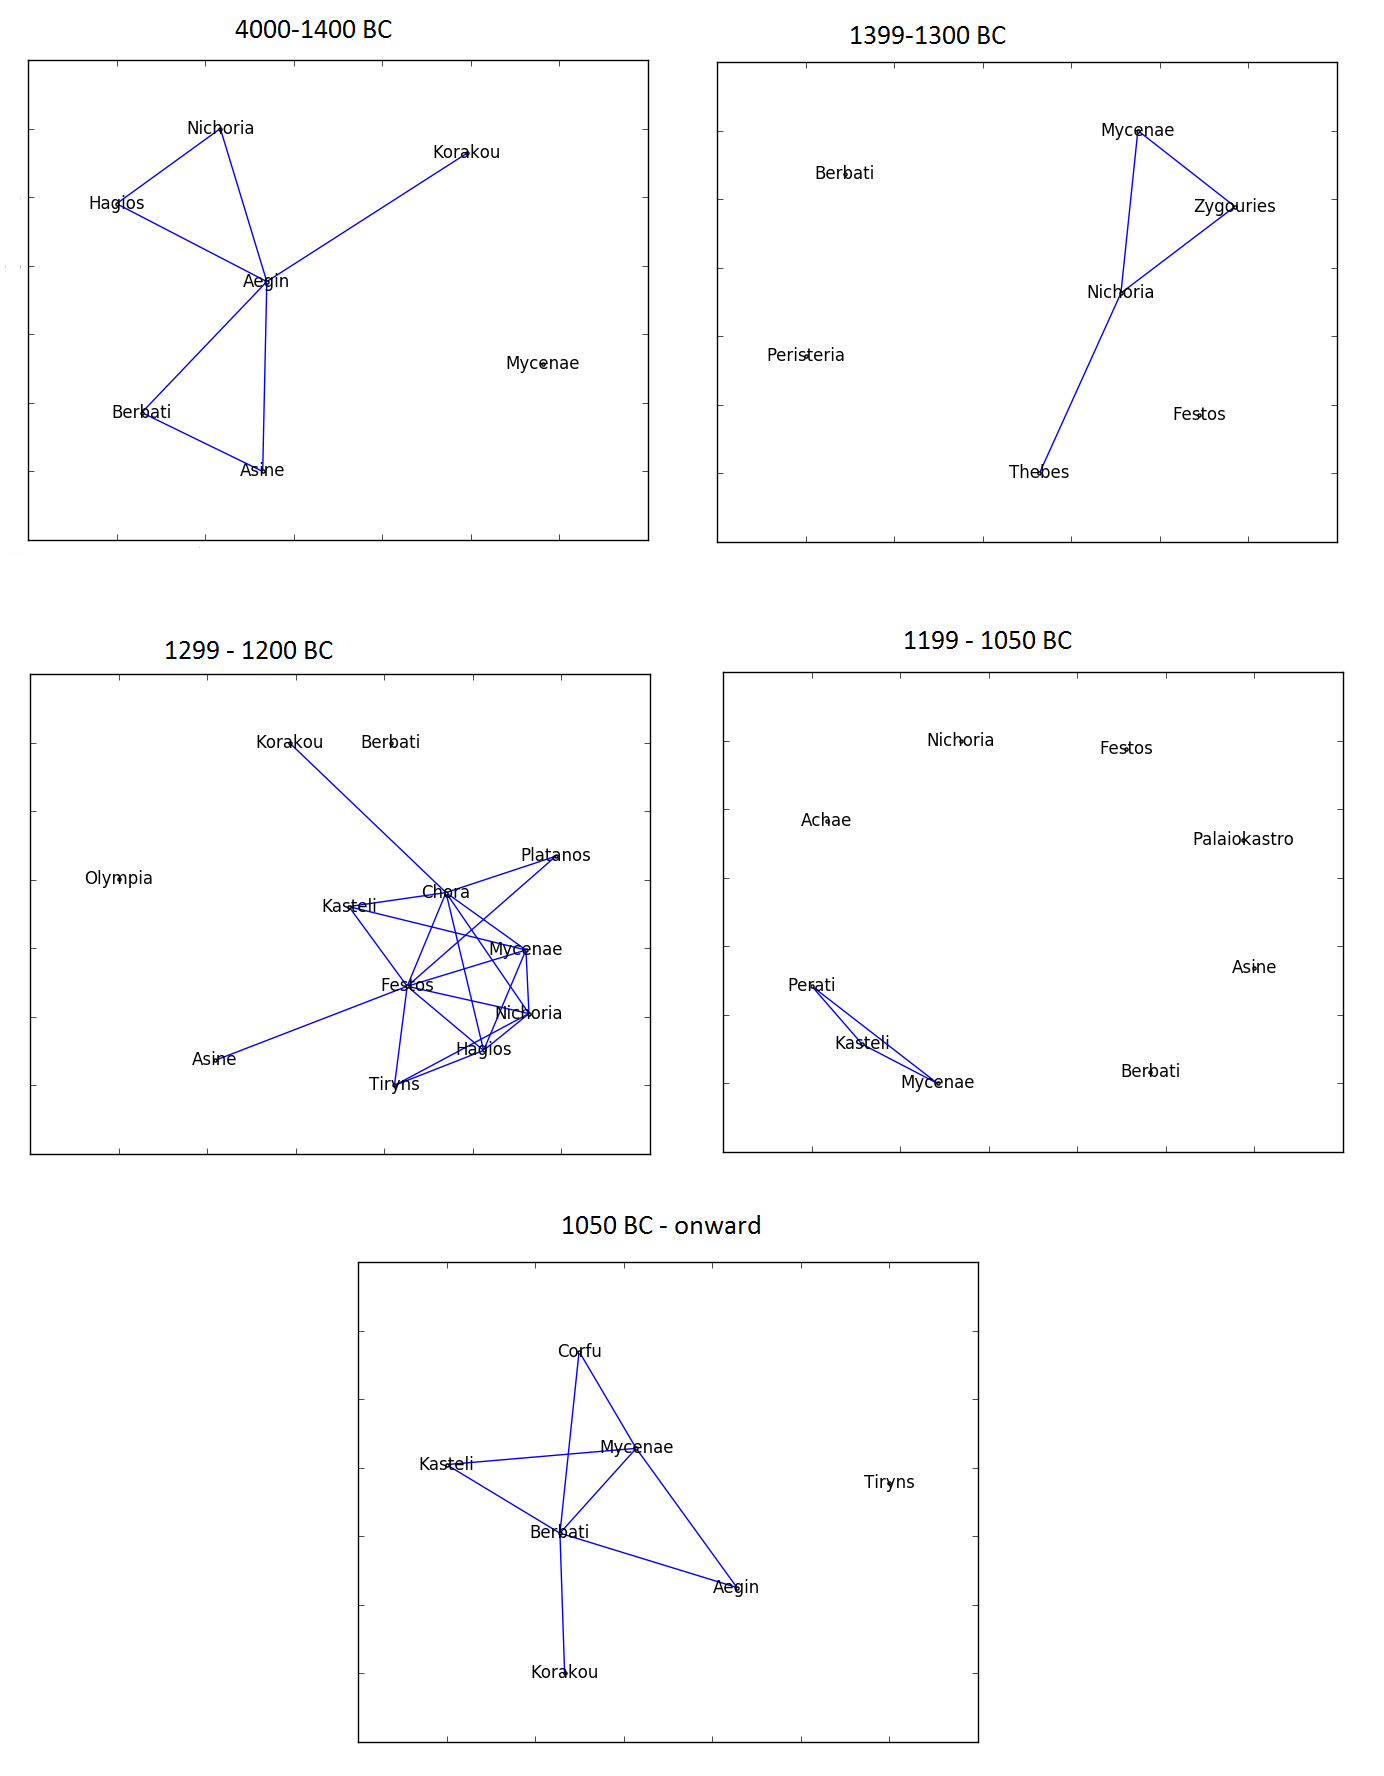
\includegraphics[width=\textwidth]{Network_evolution.png}
\caption{Evolution of networks of the Archaeological sites}
\label{fig:evolution}
\end{figure}


\begin{figure}
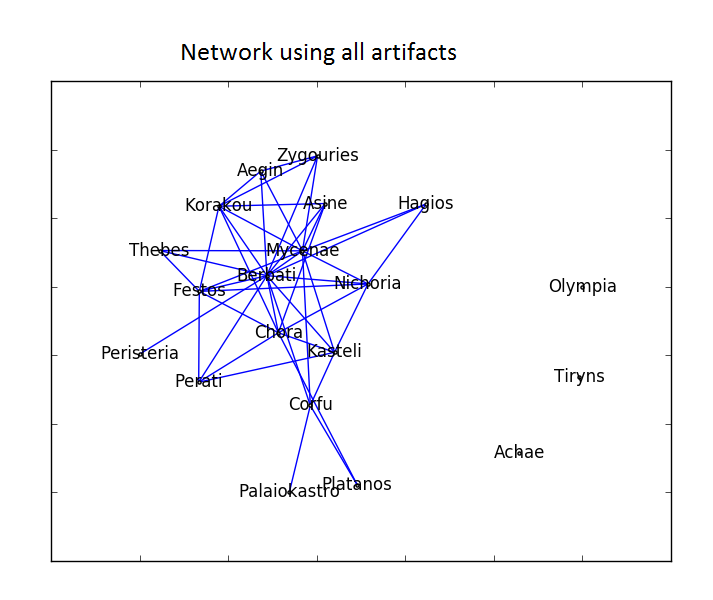
\includegraphics[width=\textwidth]{Overall_Network.png}
\caption{Overall network of the Archaeological sites}
\label{fig:overall}
\end{figure}
